% Chapter Template

\chapter{LUKS} % Main chapter title

\label{Chapitre 6.1} % Change X to a consecutive number; for referencing this chapter elsewhere, use \ref{ChapterX}

\lhead{ \emph{LUKS}} % Change X to a consecutive number; this is for the header on each page - perhaps a shortened title

%----------------------------------------------------------------------------------------
%	SECTION 1
%----------------------------------------------------------------------------------------


\section{LUKS, cryptsetup, dmcrypt}
Cryptsetup permet de gérer (lire et écrire) sur des volumes chiffrés par pain dm-crypt et LUKS. Ceci peut s'avérer fort utile lorsque les données utilisateur nécessite un degré de sécurité haut dessus de la normale.
\subsection{Mode plain dm-crypt (plain mode)}
Ce mode permet de chiffrer le périphérique secteur par secteur à l'aide d'une simple clé non-salée ou une passphrase. Aucune vérifications n'est réalisées, et aucune méta données n'est utilisée. De plus, aucune opération de formatage n'est effectuée sur les données. Lorsqu'un périphérique brut est mappé (ouvert), les opérations usuelles peuvent lui être appliquées, incluant la création de système de fichier. Les périphériques ainsi mappés sont généralement disponibles dans \textbf{/dev/mapper/<périphérique>}.
\subsection{Mode LUKS extension mode}
LUKS (Linux Unified Key Setup), est un standard de chiffrement de disque. Il ajoute un entête standardisé au début du périphérique directement suivi d'un espace de clé. Les données chiffrées sont ensuite situées juste après ces deux zones. Le tout forme un "conteneur LUKS". Le périphérique qui possède un conteneur LUKS est communément appelé "LUKS device". Dans la pluspart des cas, les deux nomenclatures peuvent désignés les deux termes. Ã noter que lorsque l'entête LUKS se situe à un offset différent de zéro, le périphérique n'est plus considéré comme un LUKS device mais comme un conteneur LUKS stoqué en mémoire. LUKS peut gérer plusieures passphrases qui peuvent être individuellement révoquées ou changées. Ceci implique un risque lors de l'utilisation de média persistant dû à l'utilisation de  bandes anti-légistes. Les passphrases sont protégées par PBKDF2 contre les attaques de type "bute-force" et dictionaire lequel implémente un hachage et un salage dans la même fonction. Chaque passphrase aussi appelée clé est associée avec l'un des 8 espace-clé. Les opérations clé qui ne sont pas liée à un espace de clé sont affectés au premier espace qui correspond à la passphrase fournie ou au premier espace vide lorsqu'un nouvelle passphrase est fournie.

Pour des raisons de sécurité, le mode "\textbf{LUKS extension}" est recommandé car il bénéficie d'une plus grande sécurité et propose la possibilité d'utiliser 8 clés différentes. Ainsi, l'utilisateur peut chiffrer 8 partitions différentes.

\subsection{Options}
\begin{description}
	\item[--hash, -h] Spécifie le hachage à utiliser lors du hachage du mot de passe. Cette option n'est utilie que lors de l'action de création. La chaîne de hachage est passée à libgcrypt ainsi tout les hashes acceptés par gcrypt sont supportés.
	\item[-key-file, -d] Utilise un fichier comme matériel de clé. Avec LUKS, le matériel de clé fourni par ce fichier via cette option sont toujours utilisés pour les passphrases existantes. Pour créer une nouvelle clé via un fichier de clé, il est nécessaire d'utiliser un argument positionel à luksFormat ou luksAddKey.
	\item[Cipher par défaut] Pour LUKS, le cipher par défaut est "aes-xts-plain64", selon la documentation.
\end{description}

\subsection{Installation}
Dans cet exercice, la partition \#3 est utilisée comme partition chiffrée. Pour ce faire, il est nécessaire d'installer au préalable le support cryptographique du noyau (\textbf{Crypt target support}). Cette option est sélectionnable dans le menu de configuration du kernel.
\begin{lstlisting}[style=Bash]
make linux-menuconfig
    Device Drivers
[*] Multiple devices driver support (RAID and LVM)
<*>   Device mapper support
<*>     Crypt target support
\end{lstlisting}
Puis installer le packet cryptsetup dans buildroot à l'aide de la commande
\begin{lstlisting}[style=Bash]
make menuconfig
    Target packages  --->
    Hardware handling  --->
[*] cryptsetup
\end{lstlisting}

Puis, le système embarqué démarré à l'aide du noyau nouvellement compilé, il est nécessaire de tester la récente installation. La partition mmcblk0p3 est donc formatée avec LUKS :
\begin{lstlisting}
# cryptsetup --key-size 256 luksFormat /dev/mmcblk0p3

WARNING!
========
This will overwrite data on /dev/mmcblk0p3 irrevocably.

Are you sure? (Type uppercase yes): YES
Enter passphrase: 
Verify passphrase: 
[   75.674159] [c0] bio: create slab <bio-1> at 1
Jan  1 00:01:12 odroidxu3 user.info kernel: [   75.674159] [c0] bio: create slab <bio-1> at 1
[   78.687741] [c5] bio: create slab <bio-1> at 1
Jan  1 00:01:15 odroidxu3 user.info kernel: [   78.687741] [c5] bio: create slab <bio-1> at 1
\end{lstlisting}

Le script qui suit permet de formater la partition \#3 au format Luks puis y place un fichier. Le script ajoute ensuite une clé et copie ensuite l'entête du fichier. Pour finir, il copie 1MB de la partition pour comparer les données.
\begin{lstlisting}[style=Bash]
#!/bin/sh

PART=/dev/mmcblk0p3
DEST=/mnt/usr
CRYPTED_VOLUME=usrfs

umount $DEST

if [ ! -d "$DEST" ];
then
        mkdir $DEST
fi

echo "[ STEP ] Creating LUKS partition on mmcblk0p3"
cryptsetup --verify-passphrase --key-size 256 luksFormat $PART

echo "[ STEP ] Copy 1 MB from the LUKS partition"   
cryptsetup luksDump $PART > 1-emptyLuks.txt

echo "[ STEP ] Setup $PART to $DEST"
cryptsetup open --type luks $PART $CRYPTED_VOLUME

ls -la /dev/mapper

echo "[ STEP ] Formatting /dev/mapper/$CRYPTED_VOLUME"
mkfs.ext4 /dev/mapper/$CRYPTED_VOLUME

echo "[ STEP ] Mounting $PART to $DEST"
mount /dev/mapper/$CRYPTED_VOLUME $DEST

echo "[ STEP ] Copying helloworld.txt to $DEST"
cp helloWorld.txt $DEST

echo "[ STEP ] Adding a new passphrase to LUKS partition"
cryptsetup -y luksAddKey $PART

echo "[ STEP ] Dumping header partition and master key"
cryptsetup luksDump $PART > 2-addKeyLuks.txt

echo "[ STEP ] Unmounting $DEST"                      
umount $DEST

echo "[ STEP ] Closing luks partition"                   
cryptsetup luksClose $CRYPTED_VOLUME
\end{lstlisting}

Les informations d'en-tête récupérées sont illustrées par le listing ci-dessous.
\begin{lstlisting}[style=Bash]
# cat 2-addKeyLuks.txt 
LUKS header information for /dev/mmcblk0p3

Version:       	1
Cipher name:   	aes
Cipher mode:   	xts-plain64
Hash spec:     	sha1
Payload offset:	4096
MK bits:       	256
MK digest:     	d6 1e ef 0b 3f 07 28 4b 85 de e3 ee 35 74 32 1d 94 fe 33 ba 
MK salt:       	26 9c d8 b7 10 68 16 6f e2 e3 4e e2 bd 32 7d 57 
               	d9 08 0d 42 e6 44 cd 82 cb fe 1d 38 3b 3f 11 01 
MK iterations: 	32500
UUID:          	58791743-f049-465c-b28f-db0d4b0dbfea

Key Slot 0: ENABLED
	Iterations:         	131551
	Salt:               	00 cf 14 3e c9 3a 34 32 d3 f1 21 cb 6f 8a 91 c1 
	                      	5a 76 29 e8 00 ac 73 ab b9 cc e5 e8 58 76 81 1b 
	Key material offset:	8
	AF stripes:            	4000
Key Slot 1: ENABLED
	Iterations:         	131281
	Salt:               	b4 30 6c 5f e9 64 ad 08 3c 08 9f 90 76 72 be 98 
	                      	ba 03 93 c6 4e 87 f0 6c 22 51 1c ca 11 0b 26 3a 
	Key material offset:	264
	AF stripes:            	4000
Key Slot 2: DISABLED
Key Slot 3: DISABLED
Key Slot 4: DISABLED
Key Slot 5: DISABLED
Key Slot 6: DISABLED
Key Slot 7: DISABLED
\end{lstlisting}
Il indique que la partition possède deux clés et que la master key dispose de 256 bits et est au format sha-1. La copie de la partition est donnée ci dessous et comparée avec les informations d'en-tête :

\begin{lstlisting}[style=Bash]
0000000 554c 534b beba 0100 6561 0073 0000 0000
0000010 0000 0000 0000 0000 0000 0000 0000 0000
0000020 0000 0000 0000 0000 7478 2d73 6c70 6961
0000030 366e 0034 0000 0000 0000 0000 0000 0000
0000040 0000 0000 0000 0000 6873 3161 0000 0000
0000050 0000 0000 0000 0000 0000 0000 0000 0000
0000060 0000 0000 0000 0000 0000 0010 0000 2000
0000070 1ed6 0bef 073f 4b28 de85 eee3 7435 1d32
0000080 fe94 ba33 9c26 b7d8 6810 6f16 e3e2 e24e
0000090 32bd 577d 08d9 420d 44e6 82cd fecb 381d
00000a0 3f3b 0111 0000 f47e 3835 3937 3731 3334
00000b0 662d 3430 2d39 3634 6335 622d 3832 2d66
00000c0 6264 6430 6234 6430 6662 6165 0000 0000
00000d0 ac00 f371 0200 df01 cf00 3e14 3ac9 3234
00000e0 f1d3 cb21 8a6f c191 765a e829 ac00 ab73
00000f0 ccb9 e8e5 7658 1b81 0000 0800 0000 a00f
0000100 ac00 f371 0200 d100 30b4 5f6c 64e9 08ad
0000110 083c 909f 7276 98be 03ba c693 874e 6cf0
0000120 5122 ca1c 0b11 3a26 0000 0801 0000 a00f
0000130 0000 adde 0000 0000 0000 0000 0000 0000
0000140 0000 0000 0000 0000 0000 0000 0000 0000
0000150 0000 0000 0000 0000 0000 0802 0000 a00f
0000160 0000 adde 0000 0000 0000 0000 0000 0000
0000170 0000 0000 0000 0000 0000 0000 0000 0000
0000180 0000 0000 0000 0000 0000 0803 0000 a00f
0000190 0000 adde 0000 0000 0000 0000 0000 0000
00001a0 0000 0000 0000 0000 0000 0000 0000 0000
00001b0 0000 0000 0000 0000 0000 0804 0000 a00f
00001c0 0000 adde 0000 0000 0000 0000 0000 0000
00001d0 0000 0000 0000 0000 0000 0000 0000 0000
00001e0 0000 0000 0000 0000 0000 0805 0000 a00f
00001f0 0000 adde 0000 0000 0000 0000 0000 0000
0000200 0000 0000 0000 0000 0000 0000 0000 0000
0000210 0000 0000 0000 0000 0000 0806 0000 a00f
0000220 0000 adde 0000 0000 0000 0000 0000 0000
0000230 0000 0000 0000 0000 0000 0000 0000 0000
0000240 0000 0000 0000 0000 0000 0807 0000 a00f
0000250 0000 0000 0000 0000 0000 0000 0000 0000
*
0001000 82c3 ffe7 35d8 7704 f5cd f39b cab4 1b9a

\end{lstlisting}
Les clés de la partition se trouvent à l'offset 0e8 pour la première et 118 pour la seconde. Il est intéressante de constater que l'offset décrit par l'en-tête correspond à l'offset par rapport aux adresses 0e0 ou 110.

\subsection{Taille de l'en-tête}
l'en-tête de la partition LUKS est représenté par la figure \ref{fig:luks partition header}. Dans le cas de cet exercice, il représente une taille de \textbf{4kB}.
\begin{figure}
	\centering
	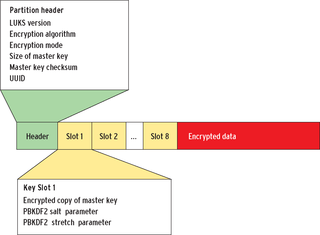
\includegraphics[width=10cm]{q5.6.3/luks-partition-header}
	\caption{\label{fig:luks partition header}En-tête de la partition LUKS}
\end{figure}
Comme le montre la copie binaire de la partition, les données chiffrées se trouvent bien à l'offset 1000 (hexa) correspondant à 4096.

Dans ce cas, chaque slot de clé possède 256 bits car la commande utilisée pour créer les clés de partition est la suivante:
\begin{lstlisting}
cryptsetup --verify-passphrase --key-size 256 luksFormat /dev/mmcblk0p3
\end{lstlisting}
De plus, "le key material offset" indique que la première clé se trouve à la position 8 et la seconde à la position 264. La différence des deux donne bien 256 B.

\subsection{Montage sur l'ordinateur hôte}
Pour pouvoir monter la partition, il est nécessaire de passer par cryptsetup qui va ouvrir la partion pour le déchiffrement. Bien entendu, il est nécessaire de connaître le mot de passe.
\begin{lstlisting}
sudo cryptsetup open --type luks /dev/mmcblk0p3 usrfs
[sudo] password for ***: 
Enter passphrase for /dev/mmcblk0p3:
sudo mount -t ext4 /dev/mapper/usrfs /media/***/usrfs/
ls -la /media/***/usrfs/
total 18
drwxr-xr-x  3 root root  1024 jun 13 06:51 .
drwxr-x---+ 3 root root  4096 jun 13 07:21 ..
-rw-r--r--  1 root root    23 jun 13 06:51 helloWorld.txt
drwx------  2 root root 12288 jun 13 06:51 lost+found
\end{lstlisting}
Ceci prouve que la partition peut être montée sur n'importe quelle machine à condition que la clé de déchiffrement soit connue.

\section{Initramfs}
U-boot propose d'utiliser initramfs mais de ce fait, il copie "bêtement" le rootfs là où devrait se trouver initramfs. Ici, l'idée est de faire les choses plus intelligente en générant un initramfs qui sera alors copié sur la \usd. u-boot le chargera ensuite dans la mémoire.

\href{http://forum.odroid.com/viewtopic.php?f=81&t=4860}{}

\subsection{uBoot}
Afin de supporter le démarrage de Initramfs, les varaibles d'environnement de uBoot doivent être modifiées. Le listing ci-dessous donne les différentes modifications à lui apporter.

\begin{lstlisting}
set initramfs_addr 0x42000000
set addmmcargs 'setenv bootargs ${bootargs} root=/dev/mmcblk0p2 rw rootwait rootfstype=ext4'
set mmcboot 'run addttyargs addmmcargs addipargs; ext2load mmc 0:1 ${fdts_addr} exynos5422-odroidxu3.dtb; ext2load mmc 0:1 ${kernel_addr} uImage; ext2load mmc 0:1 ${initramfs_addr} uInitrd; bootm ${kernel_addr} ${initramfs_addr} ${fdts_addr}'
saveenv
\end{lstlisting}
Ceci implique que \textbf{initramfs} se trouve à l'adresse \textbf{0x42000000} sur la carte \usd. Celui-là est une image au format \textbf{cpio archive} qui peut être générée manuellement.

Pour installer le support du démarrage du noyau sur initramfs, il est au préalable nécessaire de l'installer à l'aide de buildroot:
\begin{lstlisting}[style=Bash]
make linux-menuconfig
    General setup  --->
[*] Initial RAM filesystem and RAM disk (initramfs/initrd) support
(~/ses/03-labos/labo05/exercice-7/initramfs) Initramfs source file(s)
\end{lstlisting}

\subsection{Contenu}
Pour pouvoir démarrer, Initramfs à besoin d'un minimum de fichiers, lesquels sont listés ci-dessous :

\textbf{bin,dev,etc,lib,lib64,mnt/root,proc,root,sbin,sys}

\textbf{mnt/root} représente l'emplacement où sera chargé le nouveau système de fichier root. Dans le cas de cet exercice, il s'agit de \textbf{/newroot}.

\subsection{Utilité}
Cette technique peut être intéressante lorsque le système embarqué nécessite le support d'un disque dur IDE. En effet, une telle interface ne possède, dans certain cas, pas de pilote monolitique Linux. Ainsi, initramfs est un moyen très utilisé pour charger les pilotes nécessaire au noyau avant de donner la main au root file system principal. Le chargement d'un nouveau pilote est réalisé à l'aide du fichier /init de initramfs dans lequel se trouve une ligne permettant le chargement du module IDE (insmod). Ainsi, Linux saura communiquer avec le disque IDE une fois le root file system principal démarré.

Cette technique est largement répandue dans les noyau dit "exotiques" dont celui-ci ne possèderait pas tout les pilotes nativement.

\subsection{Installation dans initramfs}
L'installation de cryptsetup sur la partition initramfs nécessite plusieurs opérations, notamment la copie des librairies dynamiques permettant l'exécution de \textbf{cryptsetup} puis l'installation du module noyau appelé \textbf{dm\_mod}.

\subsubsection*{Copie des librairies nécessaires à cryptsetup}
Pour l'installation de cryptsetup dans le système initramfs, il a préalablement été nécessaire d'exécuter la commande strings filtrée sur les librairies afin d'obtenir la liste des dépendances de cryptsetup:
\begin{lstlisting}[style=Bash]
$ strings buildroot/output/target/bin/cryptsetup | grep lib
/lib/ld-linux-armhf.so.3
libcryptsetup.so.4
libuuid.so.1
libdevmapper.so.1.02
libgcrypt.so.20
libgpg-error.so.0
libpopt.so.0
libc.so.6
\end{lstlisting}

Une fois toutes les librairies identifiées, il est nécessaire de modifier le script de création de l'image initramfs afin d'y ajouter ces fichiers. Le script modifié permettant de réaliser une telle image est donné dans le listing \ref{lst:initramfs}.
\begin{lstlisting}[label=lst:initramfs,caption=Génération de l'image initramfs]
#!/bin/bash
ROOTFS_LOC=initramfs
BUILDROOT=~/ses/buildroot

if [[ -d "$ROOTFS_LOC" ]]; then
	rm -rf ${ROOTFS_LOC}
fi

mkdir $ROOTFS_LOC
mkdir -p $ROOTFS_LOC/{bin,dev,etc,home,lib,newroot,proc,root,sbin,sys}

cd $ROOTFS_LOC/dev
sudo mknod null c 1 3
sudo mknod tty c 5 0
sudo mknod console c 5 1
sudo mknod random c 1 8
sudo mknod urandom c 1 9

sudo mknod mmcblk0p b 179 0
sudo mknod mmcblk0p1 b 179 1
sudo mknod mmcblk0p2 b 179 2
sudo mknod mmcblk0p3 b 179 3
sudo mknod mmcblk0p4 b 179 4

sudo mknod ttySAC0 c 204 64
sudo mknod ttySAC1 c 204 65
sudo mknod ttySAC2 c 204 66
sudo mknod ttySAC3 c 204 67

cd ../bin
cp ${BUILDROOT}/output/target/bin/busybox .
ln -s busybox ls
ln -s busybox mkdir
ln -s busybox ln
ln -s busybox mknod
ln -s busybox mount
ln -s busybox umount
ln -s busybox sh
ln -s busybox sleep
ln -s busybox dmesg
cp ${BUILDROOT}/output/target/usr/bin/strace .
cp ${BUILDROOT}/output/target/usr/sbin/cryptsetup .
cp ${BUILDROOT}/output/target/sbin/insmod .
cp ${BUILDROOT}/output/target/sbin/lsmod .
cp ${BUILDROOT}/output/target/sbin/modprobe .

cd ../sbin
ln -s ../bin/busybox switch_root

cd ../lib
cp ${BUILDROOT}/output/target/lib/libc-2.19-2014.08.so .
cp ${BUILDROOT}/output/target/lib/ld-2.19-2014.08.so .
cp ${BUILDROOT}/output/target/usr/lib/libcryptsetup.so.4.6.0 .
cp ${BUILDROOT}/output/target/lib/libuuid.so.1.3.0 .
cp ${BUILDROOT}/output/target/usr/lib/libdevmapper.so.1.02 .
cp ${BUILDROOT}/output/target/usr/lib/libgcrypt.so.20.0.2 .
cp ${BUILDROOT}/output/target/usr/lib/libgpg-error.so.0.10.0 .
cp ${BUILDROOT}/output/target/usr/lib/libpopt.so.0.0.0 .
cp ${BUILDROOT}/output/target/lib/libpthread.so.0 .

ln -s libc-2.19-2014.08.so libc.so.6
ln -s ld-2.19-2014.08.so ld-linux-armhf.so.3
ln -s libcryptsetup.so.4.6.0 libcryptsetup.so.4
ln -s libuuid.so.1.3.0 libuuid.so.1
ln -s libgcrypt.so.20.0.2 libgcrypt.so.20
ln -s libgpg-error.so.0.10.0 libgpg-error.so.0
ln -s libpopt.so.0.0.0 libpopt.so.0
ln -s . arm-linux-gnueabihf

cd ..

cat << EOT >> init
#!/bin/busybox sh
mount -t proc none /proc
mount -t sysfs none /sys

. ./home/mountLuks

umount /proc
umount /sys

exec sh
# exec switch_root /newroot /init
EOT

chmod 755 ./init

cd ..

. ./postInstall

sudo chown -R 0:0 $ROOTFS_LOC

cd $ROOTFS_LOC
find . | cpio --quiet -o -H newc > ../Initrd

cd ..

gzip -9 -c Initrd > Initrd.gz

mkimage -A arm -T ramdisk -C none -d Initrd.gz uInitrd
\end{lstlisting}

Le script qui suit est appelé par le précédent et génère le script qui sera appelé par initramfs afin de monter la partition chiffrée.
\begin{lstlisting}[label=lst:luks initramfs,caption=Montage de la partition chiffrée]
#!/bin/bash

echo "#########################################################################"
echo "# Initramfs image post installation script                              #"
echo "#                                                                       #"
echo "# Author: Jonathan Worreth                                              #"
echo "# Date: 08 May 2015                                                     #"
echo "#                                                                       #"
echo "# This script creates passphrase file which will be copied to the       #"
echo "# the initram file system. It generates a script which will mount the   #"
echo "# crypted part on the target.                                           #"
echo "#                                                                       #"
echo "#########################################################################"

cd ${ROOTFS_LOC}/home

if [[ -f passphrase ]]; then
	rm passphrase
fi

dd if=/dev/urandom of=passphrase bs=1 count=64
chmod 400 passphrase

cat << EOT >> mountLuks
#!/bin/busybox sh

PART=/dev/mmcblk0p2
DEST=/newroot
CRYPTED_VOLUME=rootfs

echo "[ STEP ] Setup \$PART to \$DEST"
cryptsetup open --type luks --key-file home/passphrase \$PART \$CRYPTED_VOLUME

echo "[ STEP ] Mounting \$PART to \$DEST"
mount /dev/mapper/\$CRYPTED_VOLUME \$DEST
EOT

chmod 500 ./mountLuks

cd ../..
\end{lstlisting}

\subsection{Exécution}
Une fois la carte prète à l'exécution, elle a été introduite dans l'Odroid et celui-ci démarré. Le résultat du chargement de Initramfs est donné ci-dessous :
\begin{lstlisting}[style=Bash]
[ STEP ] Setup /dev/mmcblk0p2 to /newroot
[   10.975193] [c6] bio: create slab <bio-1> at 1
[   11.201114] [c7] bio: create slab <bio-1> at 1
[ STEP ] Mounting /dev/mmcblk0p2 to /newroot
[   11.212956] [c7] EXT4-fs (dm-0): couldn't mount as ext3 due to feature incompatibilities
[   11.220194] [c7] EXT4-fs (dm-0): couldn't mount as ext2 due to feature incompatibilities
[   11.327879] [c7] EXT4-fs (dm-0): recovery complete
[   11.332869] [c7] EXT4-fs (dm-0): mounted filesystem with ordered data mode. Opts: (null)
sh: can't access tty; job control turned off
\end{lstlisting}

Ces résultats montrent clairement que la partition a été montée avec succès car elle contient les fichiers suivants :

\begin{lstlisting}[style=Bash]
/ # ls /newroot
bin         home        linuxrc     mnt         root        tmp
dev         lib         lost+found  opt         sbin        usr
etc         lib32       media       proc        sys         var
\end{lstlisting}

Pour démarré ne nouveau rootfs, la commande illustrée dans le listing \ref{lst:switch root} a été exécutée et son résultat joint au listing.
\begin{lstlisting}[label={lst:switch root},caption=Changement de root file system]
/ # exec switch_root /newroot /sbin/init
can't open /dev/null: No such file or directory
can't open /dev/null: No such file or directory
can't open /dev/null: No such file or directory
can't open /dev/null: No such file or directory
can't open /dev/null: No such file or directory
can't open /dev/null: No such file or directory
Starting logging: OK
Jan  1 00:13:55 odroidxu3 syslog.info syslogd started: BusyBox v1.22.1
Jan  1 00:13:55 odroidxu3 user.notice kernel: klogd started: BusyBox v1.22.1 (2015-05-21 16:20:39 CEST)
Jan  1 00:13:55 odroidxu3 user.info kernel: [    0.000000] [c0] Booting Linux on physical CPU 0x100
Jan  1 00:13:55 odroidxu3 user.info kernel: [    0.000000] [c0] Initializing cgroup subsys cpu
Jan  1 00:13:55 odroidxu3 user.info kernel: [    0.000000] [c0] Initializing cgroup subsys cpuacct
Jan  1 00:13:55 odroidxu3 user.notice kernel: [    0.000000] [c0] Linux version 3.10.63 (embedhfw@experiment) (gcc version 4.9.2 20140904 (prerelease) (crosstool-NG linaro-1.13.1-4.9-2014.09 - Linaro GCC 4.9-5
Jan  1 00:13:55 odroidxu3 user.warn kernel: [    0.000000] [c0] CPU: ARMv7 Processor [410fc073] revision 3 (ARMv7), cr=10c5387d
Jan  1 00:13:55 odroidxu3 user.warn kernel: [    0.000000] [c0] CPU: PIPT / VIPT nonaliasing data cache, VIPT aliasing instruction cache
Jan  1 00:13:55 odroidxu3 user.info kernel: [    0.000000] [c0] Machine: ODROID-XU3, model: Hardkernel odroid-xu3 board based on EXYNOS5422
Jan  1 00:13:55 odroidxu3 user.info kernel: [    0.000000] [c0] ION: Contiguous 0x6650000 bytes @ 0x0 defined for 0:common
Jan  1 00:13:55 odroidxu3 user.info kernel: [    0.000000] [c0] ION: Contiguous 0x400000 bytes @ 0x0 defined for 2:mfc_sh
Jan  1 00:13:55 odroidxu3 user.info kernel: [    0.000000] [c0] ION: Contiguous 0x800000 bytes @ 0x0 defined for 10:g2d_wfd
Jan  1 00:13:55 odroidxu3 user.info kernel: [    0.000000] [c0] ION: Contiguous 0x6000000 bytes @ 0x0 defined for 11:video
Jan  1 00:13:55 odroidxu3 user.info kernel: [    0.000000] [c0] ION: Contiguous 0x1000000 bytes @ 0x0 defined for 7:mfc_input
Jan  1 00:13:55 odroidxu3 user.info kernel: [    0.000000] [c0] ION: Contiguous 0x400000 bytes @ 0x0 defined for 9:sectbl
Jan  1 00:13:55 odroidxu3 user.info kernel: [    0.000000] [c0] ION: Contiguous 0x400000 bytes @ 0x0 defined for 8:mfc_fw
Jan  1 00:13:55 odroidxu3 user.info kernel: [    0.000000] [c0] ION: Contiguous 0x400000 bytes @ 0x0 defined for 12:mfc_nfw
Jan  1 00:13:55 odroidxu3 user.info kernel: [    0.000000] [c0] ION: Contiguous 0x400000 bytes @ 0x0 defined for 13:secdma
Jan  1 00:13:55 odroidxu3 user.info kernel: [    0.000000] [c0] cma: CMA: reserved 104 MiB at b8000000
Jan  1 00:13:55 odroidxu3 user.info kernel: [    0.000000] [c0] cma: CMA: reserved 4 MiB at b7c00000
Jan  1 00:13:55 odroidxu3 user.info kernel: [    0.000000] [c0] cma: CMA: reserved 8 MiB at b7400000
Jan  1 00:13:55 odroidxu3 user.info kernel: [    0.000000] [c0] cma: CMA: reserved 96 MiB at b1400000
Starting mdev...
Jan  1 00:13:55 odroidxu3 user.info kernel: [    0.000000] [c0] cma: CMA: reserved 16 MiB at b0400000
Jan  1 00:13:55 odroidxu3 user.info kernel: [    0.000000] [c0] cma: CMA: reserved 4 MiB at b0000000
Jan  1 00:13:55 odroidxu3 user.info kernel: [    0.000000] [c0] cma: CMA: reserved 4 MiB at afc00000
Jan  1 00:13:55 odroidxu3 user.info kernel: [    0.000000] [c0] cma: CMA: reserved 4 MiB at af800000
Jan  1 00:13:55 odroidxu3 user.info kernel: [    0.000000] [c0] cma: CMA: reserved 4 MiB at af400000
Jan  1 00:13:55 odroidxu3 user.info kernel: [    0.000000] [c0] cma: CMA: reserved 256 MiB at 5f800000
Jan  1 00:13:55 odroidxu3 user.warn kernel: [    0.000000] [c0] Memory policy: ECC disabled, Data cache writealloc
Jan  1 00:13:55 odroidxu3 user.info kernel: [    0.000000] [c0] create_mapping_memory: section: 40000000 ~ 6f800000
Jan  1 00:13:55 odroidxu3 user.warn kernel: [    0.000000] [c0] CPU EXYNOS5422 (id 0xe5422001)
/etc/init.d/S10mdev: line 19: can't create /proc/sys/kernel/hotplug: nonexistent directory
Jan  1 00:13:55 odroidxu3 user.debug kernel: [    0.000000] [c0] free_area_init_node: node 0, pgdat c097ab80, node_mem_map c0de2000
Jan  1 00:13:55 odroidxu3 user.debug kernel: [    0.000000] [c0]   Normal zone: 1520 pages used for memmap
Jan  1 00:13:55 odroidxu3 user.debug kernel: [    0.000000] [c0]   Normal zone: 0 pages reserved
Jan  1 00:13:55 odroidxu3 user.debug kernel: [    0.000000] [c0]   Normal zone: 194560 pages, LIFO Jan  1 00:13:5Jan  1 00:13:5Jan  1 00:13:5Jan  1 00:13:5Jan  1 00:13:5Jan  1 00:13:5mdev: /sys/class: No suchy
Starting network...
ip: RTNETLINK answers: File exists
ifup: can't open '/var/run/ifstate': No such file or directory
Couldn't open /dev/null: No such file or directory
Starting sshd: Couldn't open /dev/null: No such file or directory
touch: /var/lock/sshd: No such file or directory
OK
/etc/init.d/S90fan_low_speed: line 2: can't create /sys/class/pwm/pwmchip0/export: nonexistent directory
/etc/init.d/S90fan_low_speed: line 3: can't create /sys/class/pwm/pwmchip0/pwm0/period: nonexistent directory
/etc/init.d/S90fan_low_speed: line 4: can't create /sys/class/pwm/pwmchip0/pwm0/duty_cycle: nonexistent directory
/etc/init.d/S90fan_low_speed: line 5: can't create /sys/class/pwm/pwmchip0/pwm0/enable: nonexistent directory
/etc/init.d/S90fan_low_speed: line 6: can't create /sys/class/pwm/pwmchip0/unexport: nonexistent directory
can't open /dev/ttySAC2: No such file or directory
Jan  1 00:13:56 odroidxu3 daemon.info init: can't open /dev/ttySAC2: No such file or directory
Jan  1 00:13:57 odroidxu3 daemon.info init: process '/sbin/getty -L  ttySAC2 115200 vt100 ' (pid 1660) exited. Scheduling for restart.
\end{lstlisting}

\subsection{Analyse des résultats}
La première chose à constater est que le script \textbf{init} exécuté n'est probablement pas le bon car les noeuds dont il a besoin ne sont pas disponibles. Il s'agit de :
\begin{description}
	\item[/dev/null]
	\item[/var/run/ifstate]
	\item[/var/loc/sshd]
	\item[/dev/ttySAC2]
\end{description}
Une alternative a ce problème est de démarrer la commande \textbf{sh} à la place de démarrer \textbf{/sbin/init} en modifiant la commande ainsi:
\begin{lstlisting}
exec switch_root /newroot /sbin/sh
\end{lstlisting}
Qui ne démarre aucun démon ni logiciel mais qui permet de travailler sur le nouveau rootfs.

\subsection{Démarrage automatique}
Pour réaliser un démarrage automatique du nouveau root file system il suffit de modifier la ligne
\begin{lstlisting}
exec sh
\end{lstlisting}
qui devient
\begin{lstlisting}
exec switch_root /newroot /sbin/init
\end{lstlisting}

qui produit les mêmes résultats que précédemment, à une différence près : La ligne 8 qui n'affiche pas la commande exécutée (\textbf{exec switch\_root /newroot /sbin/init})
\begin{lstlisting}[numbers=left]
[ STEP ] Setup /dev/mmcblk0p2 to /newroot
[   11.027084] [c7] bio: create slab <bio-1> at 1
[   11.247513] [c4] bio: create slab <bio-1> at 1
[ STEP ] Mounting /dev/mmcblk0p2 to /newroot
[   11.259272] [c4] EXT4-fs (dm-0): couldn't mount as ext3 due to feature incompatibilities
[   11.266512] [c4] EXT4-fs (dm-0): couldn't mount as ext2 due to feature incompatibilities
[   11.284174] [c4] EXT4-fs (dm-0): mounted filesystem with ordered data mode. Opts: (null)
can't open /dev/null: No such file or directory
can't open /dev/null: No such file or directory
can't open /dev/null: No such file or directory
can't open /dev/null: No such file or directory
can't open /dev/null: No such file or directory
can't open /dev/null: No such file or directory
Starting logging: OK
Jan  1 00:00:07 odroidxu3 syslog.info syslogd started: BusyBox v1.22.1
Jan  1 00:00:07 odroidxu3 user.notice kernel: klogd started: BusyBox v1.22.1 (2015-05-21 16:20:39 CEST)
Jan  1 00:00:07 odroidxu3 user.info kernel: [    0.000000] [c0] Booting Linux on physical CPU 0x100
Jan  1 00:00:07 odroidxu3 user.info kernel: [    0.000000] [c0] Initializing cgroup subsys cpu
Jan  1 00:00:07 odroidxu3 user.info kernel: [    0.000000] [c0] Initializing cgroup subsys cpuacct
Jan  1 00:00:07 odroidxu3 user.notice kernel: [    0.000000] [c0] Linux version 3.10.63 (embedhfw@experiment) (gcc version 4.9.2 20140904 (prerelease) (crosstool-NG linaro-1.13.1-4.9-2014.09 - Linaro GCC 4.9-5
Jan  1 00:00:07 odroidxu3 user.warn kernel: [    0.000000] [c0] CPU: ARMv7 Processor [410fc073] revision 3 (ARMv7), cr=10c5387d
Jan  1 00:00:07 odroidxu3 user.warn kernel: [    0.000000] [c0] CPU: PIPT / VIPT nonaliasing data cache, VIPT aliasing instruction cache
Jan  1 00:00:07 odroidxu3 user.info kernel: [    0.000000] [c0] Machine: ODROID-XU3, model: Hardkernel odroid-xu3 board based on EXYNOS5422
Jan  1 00:00:07 odroidxu3 user.info kernel: [    0.000000] [c0] ION: Contiguous 0x6650000 bytes @ 0x0 defined for 0:common
Jan  1 00:00:07 odroidxu3 user.info kernel: [    0.000000] [c0] ION: Contiguous 0x400000 bytes @ 0x0 defined for 2:mfc_sh
Jan  1 00:00:07 odroidxu3 user.info kernel: [    0.000000] [c0] ION: Contiguous 0x800000 bytes @ 0x0 defined for 10:g2d_wfd
Jan  1 00:00:07 odroidxu3 user.info kernel: [    0.000000] [c0] ION: Contiguous 0x6000000 bytes @ 0x0 defined for 11:video
Jan  1 00:00:07 odroidxu3 user.info kernel: [    0.000000] [c0] ION: Contiguous 0x1000000 bytes @ 0x0 defined for 7:mfc_input
Starting mdev...
Jan  1 00:00:07 odroidxu3 user.info kernel: [    0.000000] [c0] ION: Contiguous 0x400000 bytes @ 0x0 defined for 9:sectbl
Jan  1 00:00:07 odroidxu3 user.info kernel: [    0.000000] [c0] ION: Contiguous 0x400000 bytes @ 0x0 defined for 8:mfc_fw
Jan  1 00:00:07 odroidxu3 user.info kernel: [    0.000000] [c0] ION: Contiguous 0x400000 bytes @ 0x0 defined for 12:mfc_nfw
Jan  1 00:00:07 odroidxu3 user.info kernel: [    0.000000] [c0] ION: Contiguous 0x400000 bytes @ 0x0 defined for 13:secdma
Jan  1 00:00:07 odroidxu3 user.info kernel: [    0.000000] [c0] cma: CMA: reserved 104 MiB at b8000000
Jan  1 00:00:07 odroidxu3 user.info kernel: [    0.000000] [c0] cma: CMA: reserved 4 MiB at b7c00000
Jan  1 00:00:07 odroidxu3 user.info kernel: [    0.000000] [c0] cma: CMA: reserved 8 MiB at b7400000
Jan  1 00:00:07 odroidxu3 user.info kernel: [    0.000000] [c0] cma: CMA: reserved 96 MiB at b1400000
/etc/init.d/S10mdev: line 19: Jan  1 00:00:07 odroidxu3 user.info kernel: [    0.000000] [c0] cma: CMA: reserved 16 MiB at b0400000
can't create /proc/sys/kernel/hotplug: nonexistent directory
Jan  1 00:00:07 odroidxu3 user.info kernel: [    0.000000] [c0] cma: CMA: reserved 4 MiB at b0000000
Jan  1 00:00:07 odroidxu3 user.info kernel: [    0.000000] [c0] cma: CMA: reserved 4 MiB at afc00000
Jan  1 00:00:07 odroidxu3 user.info kernel: [    0.000000] [c0] cma: CMA: reserved 4 MiB at af800000
Jan  1 00:00:07 odroidxu3 user.info kernel: [    0.000000] [c0] cma: CMA: reserved 4 MiB at af400000
Jan  1 00:00:07 odroidxu3 user.info kernel: [    0.000000] [c0] cma: CMA: reserved 256 MiB at 5f800000
Jan  1 00:00:07 odroidxu3 user.warn kernel: [    0.000000] [c0] Memory policy: ECC disabled, Data cache writealloc
Jan  1 00:00:07 odroidxu3 user.info kernel: [    0.000000] [c0] create_mapping_memory: section: 40000000 ~ 6f800000
Jan  1 00:00:07 odroidxu3 user.warn kernel: [    0.000000] [c0] CPU EXYNOS5422 (id 0xe5422001)
Jan  1 00:00:07 odroidxu3 user.debug kernel: [    0.000000] [c0] On node 0 totalpages: 518656
Jan  1 00:00:07 odroidxu3 user.debug kernel: [    0.000000] [c0] free_area_init_node: node 0, pgdat c097ab80, node_mem_map c0de2000
Jan  1 00:00:07 odroidxu3 user.debug kernel: [    0.000000] [c0]   Normal zone: 1520 pages used for memmap
Jan  1 00:00:07 odroidxu3 user.debug kernel: [    0.000000] [c0]   Normal zone: 0 pages reserJan  1 00:00:0Jan  1 00:00:0Jan  1 00:00:0Jan  1 00:00:0Jan  1 00:00:0mdev: /sys/class: No such file or directory
Starting network...
ip: RTNETLINK answers: File exists
ifup: can't open '/var/run/ifstate': No such file or directory
Couldn't open /dev/null: No such file or directory
Starting sshd: Couldn't open /dev/null: No such file or directory
touch: /var/lock/sshd: No such file or directory
OK
/etc/init.d/S90fan_low_speed: line 2: can't create /sys/class/pwm/pwmchip0/export: nonexistent directory
/etc/init.d/S90fan_low_speed: line 3: can't create /sys/class/pwm/pwmchip0/pwm0/period: nonexistent directory
/etc/init.d/S90fan_low_speed: line 4: can't create /sys/class/pwm/pwmchip0/pwm0/duty_cycle: nonexistent directory
/etc/init.d/S90fan_low_speed: line 5: can't create /sys/class/pwm/pwmchip0/pwm0/enable: nonexistent directory
/etc/init.d/S90fan_low_speed: line 6: can't create /sys/class/pwm/pwmchip0/unexport: nonexistent directory
can't open /dev/ttySAC2: No such file or directory
Jan  1 00:00:07 odroidxu3 daemon.info init: can't open /dev/ttySAC2: No such file or directory
Jan  1 00:00:08 odroidxu3 daemon.info init: process '/sbin/getty -L  ttySAC2 115200 vt100 ' (pid 1656) exited. Scheduling for restart.
\end{lstlisting}
